% -*- coding: utf-8; -*-

\chapter{Aplicação da Compressão Horizontal}
\label{cap:aplicacao_tec}

Como apresentado na Seção \ref{sec:comp_hor}, a CH adiciona algumas informações à prova antes da e durante a compressão, essas informações são posteriormente utilizadas na validação da derivação compactada. A CH só é realmente efetiva na compactação se executar uma certa quantidade de colapsos durante a compressão. A prova da Figura \ref{fig:exe_gra_pro}, por exemplo, não contém nenhum par de vértices a ser colapsado, nesse caso, a aplicação da CH resultaria no aumento do espaço necessário para representar a prova.

Para exemplificar a aplicação da CH, considere a prova da seguinte fórmula denominada $Fib_4$ (Figura \ref{fig:prova_fib_4}) $$((A1 \supset A2) \supset ((A1 \supset (A2 \supset A3)) \supset ((A2 \supset (A3 \supset A4)) \supset (A1 \supset A4))))$$ que na representação de grafos direcionados contém 17 vértices, sendo que 7 deles serão colapsados durante a compressão.

\begin{figure}[ht]
    \begin{center}
        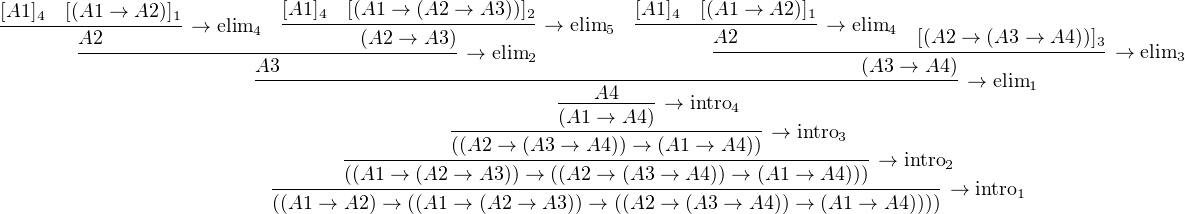
\includegraphics[height=80pt,width=400pt]{images/prooftree0x.png}
    \caption{Prova da fórmula $Fib_{4}$}
    \label{fig:prova_fib_4}
    \end{center}
\end{figure}

\begin{figure}[!ht]
    \begin{center}
        \begin{tikzpicture}[state/.style={rectangle, inner sep=5pt},  node distance=1cm]
            % \tikzstyle{every state}=[circle,thick,minimum size=5mm, text=black,minimum width=1cm]
            \node[state] (C1) {$((A1 \supset A2) \supset ((A1 \supset (A2 \supset A3)) \supset ((A2 \supset (A3 \supset A4)) \supset (A1 \supset A4))))$};
            \node[state] (C2) [above = 0.7cm of C1] {$((A1 \supset (A2 \supset A3)) \supset ((A2 \supset (A3 \supset A4)) \supset (A1 \supset A4)))$};
            \node[state] (C3) [above = 0.7cm of C2] {$((A2 \supset (A3 \supset A4)) \supset (A1 \supset A4))$};
            \node[state] (C4) [above = 0.7cm of C3] {$(A1 \supset A4)$};
            \node[state] (C5) [above = 0.7cm of C4] {$A4$};
            \node[state] (A3) [above left = 0.7cm and 3.2cm of C5] {$A3$};
            \node[state] (A3A4) [above right = 0.7cm and 3.2cm of C5] {$(A3 \supset A4)$};
            \node[state] (A2) [above left = 0.7cm and 1cm of A3] {$A2$};
            \node[state] (A2A3) [above right = 0.7cm and 1cm of A3] {$(A2 \supset A3)$};
            \node[state] (A1_1) [above left = 0.7cm and -0.3cm of A2] {$A1$};
            \node[state] (A1A2_1) [above right = 0.7cm and -0.3cm of A2] {$(A1 \supset A2)$};
            \node[state] (A1_2) [above left = 0.7cm and -0.8cm of A2A3] {$A1$};
            \node[state] (A1A2A3) [above right = 0.7cm and -1.2cm of A2A3] {$A1 \supset (A2 \supset A3)$};
            \node[state] (A2_2) [above left = 0.7cm and 0.5cm of A3A4] {$A2$};
            \node[state] (A2A3A4) [above right = 0.7cm and -2.5cm of A3A4] {$A2 \supset (A3 \supset A4)$};
            \node[state] (A1_3) [above left = 0.7cm and -0.3cm of A2_2] {$A1$};
            \node[state] (A1A2_2) [above right = 0.7cm and -0.3cm of A2_2] {$(A1 \supset A2)$};
            
            \path[-latex]  (C2) edge [thick, left] (C1);
            \path[-latex]  (C3) edge [thick, left] (C2);
            \path[-latex]  (C4) edge [thick, left] (C3);
            \path[-latex]  (C5) edge [thick, left] (C4);
            \path[-latex]  (A3) edge [thick, left] (C5);
            \path[-latex]  (A3A4) edge [thick, left] (C5);
            \path[-latex]  (A2) edge [thick, left] (A3);
            \path[-latex]  (A2A3) edge [thick, left] (A3);
            \path[-latex]  (A1_1) edge [thick, left] (A2);
            \path[-latex]  (A1A2_1) edge [thick, left] (A2);
            \path[-latex]  (A1_2) edge [thick, left] (A2A3);
            \path[-latex]  (A1A2A3) edge [thick, left] (A2A3);
            \path[-latex]  (A2_2) edge [thick, left] (A3A4);
            \path[-latex]  (A2A3A4) edge [thick, left] (A3A4);
            \path[-latex]  (A1_3) edge [thick, left] (A2_2);
            \path[-latex]  (A1A2_2) edge [thick, left] (A2_2);
            
            % \path[-latex]  (a1_2) edge [thick, left] node {0} (a2_2);
            % \path[-latex]  (a1a2_2) edge [thick, right] node {0} (a2_2);
            % \path[-latex]  (a2_2) edge [thick, left] node {0} (a3a4);
            % \path[-latex]  (a3a4) edge [thick, left, dotted] (sa3a4);
        \end{tikzpicture}
        \caption{EGDD da derivação de $Fib_4$}
        \label{fig:der_fib4}
    \end{center}
\end{figure}

Neste Capítulo utilizamos como métrica para o tamanho de uma prova o tamanho do grafo direcionado que o representa (\textit{quantidade de vértices} $+$ \textit{quantidade de arestas}).

O grafo que representa a prova de $Fib_4$ possui tamanho 40 (17 \textit{vértices} $+$ 16 \textit{arestas dedutivas} $+$ 7 \textit{arestas de descarte}), antes de iniciar a compressão, as arestas de descarte são substituídas pelas cadeias de bits de dependências associadas a cada aresta dedutiva, logo, o tamanho do grafo antes de inciar a compressão é 33.

% Na dedutiva, o t. A representação em DOT da prova possui xxx caracteres.aresta compressão da prova de $Fib_4$ são executados 4 colapsos de vértices. Considerando o nível da conclusão como o nível 1, até o nível 6 nenhum colapso é realizado; no nível 7, existem 2 vértices rotulados com 'A2' resultando em 1 colapso; no nível 8, existem 3 vértices rotulados com 'A2' resultando em 2 colapsos e existem 2 vértices rotulados com '$A1 \supset A2$' resultando em 1 colapso.

Considerando o nível da conclusão como o nível 1, o primeiro colapso é realizado no nível 7 entre os 2 vértices rotulados com a fórmula 'A2'.

\begin{center}
    \begin{tikzpicture}[state/.style={rectangle, inner sep=5pt},  node distance=1cm]
        % \tikzstyle{every state}=[circle,thick,minimum size=5mm, text=black,minimum width=1cm]
        \node[state] (a3) {$A3$};
        \node[circle,fill,inner sep=1.5pt] (sa3) [below = 1cm of a3] {};
        \node[state] (a2_1) [above = 1cm of a3] {$\boldsymbol{A2}$};
        \node[state] (a1_1) [above left = 1.25cm and 0cm of a2_1] {$A1$};
        \node[state] (a1a2_1) [above right = 1.25cm and 0cm of a2_1] {$A1 \mysupset A2$};
        
        \node[state] (a3a4) [right = 4cm of a3] {$A3 \supset A4$};
        \node[circle,fill,inner sep=1.5pt] (sa3a4) [below = 1cm of a3a4] {};
        \node[state] (a2_2) [above = 1cm of a3a4] {$\boldsymbol{A2}$};
        \node[state] (a1_2) [above left = 1.25cm and 0cm of a2_2] {$A1$};
        \node[state] (a1a2_2) [above right = 1.25cm and 0cm of a2_2] {$A1 \mysupset A2$};
        
        \path[-latex]  (a1_1) edge [thick, left] node {0} (a2_1);
        \path[-latex]  (a1a2_1) edge [thick, right] node {0} (a2_1);
        \path[-latex]  (a2_1) edge [thick, left] node {0} (a3);
        \path[-latex]  (a3) edge [thick, left, dotted] (sa3);
        
        \path[-latex]  (a1_2) edge [thick, left] node {0} (a2_2);
        \path[-latex]  (a1a2_2) edge [thick, right] node {0} (a2_2);
        \path[-latex]  (a2_2) edge [thick, left] node {0} (a3a4);
        \path[-latex]  (a3a4) edge [thick, left, dotted] (sa3a4);
    \end{tikzpicture}
\end{center}

\noindent Como ambos os vértices possuem 2 premissas e ainda não foram colapsados, são adicionadas 4 arestas de ancestralidade.

\begin{center}
    \begin{tikzpicture}[state/.style={rectangle, inner sep=5pt},  node distance=1cm]
        % \tikzstyle{every state}=[circle,thick,minimum size=5mm, text=black,minimum width=1cm]
        \node[state] (a2) {$\boldsymbol{A2}$};
        
        \node[state] (a3) [below left = 1.25cm and 0cm of a2] {$A3$};
        \node[state] (a3a4) [below right = 1.25cm and 0cm of a2] {$A3 \supset A4$};
        \node[circle,fill,inner sep=1.5pt] (sa3) [below = 1cm of a3] {};
        \node[circle,fill,inner sep=1.5pt] (sa3a4) [below = 1cm of a3a4] {};
        
        \node[state] (a1_1) [above left = 1.25cm and 2cm of a2] {$A1$};
        \node[state] (a1a2_1) [above left = 1.25cm and 0.1cm of a2] {$A1 \mysupset A2$};
        \node[state] (a1_2) [above right = 1.25cm and 0.1cm of a2] {$A1$};
        \node[state] (a1a2_2) [above right = 1.25cm and 2cm of a2] {$A1 \mysupset A2$};
        
        \path[-latex]  (a1_1) edge [thick, left] node {0} (a2);
        \path[-latex]  (a1a2_1) edge [thick, right] node {0} (a2);
        \path[-latex]  (a2) edge [thick, left] node {1} (a3);
        \path[-latex]  (a3) edge [thick, left, dotted] (sa3);
        
        \path[-latex]  (a1_2) edge [thick, left] node {0} (a2);
        \path[-latex]  (a1a2_2) edge [thick, right] node {0} (a2);
        \path[-latex]  (a2) edge [thick, right] node {2} (a3a4);
        \path[-latex]  (a3a4) edge [thick, left, dotted] (sa3a4);
        
        \path[-latex] (a3) edge [thick, left, dashed, bend left=20] node {0;1} (a1_1);
        \path[-latex] (a3) edge [thick, left, dashed, bend left=10] node {0;1} (a1a2_1);
        
        \path[-latex] (a3a4) edge [thick, right, dashed, bend right=10] node {0;2} (a1_2);
        \path[-latex] (a3a4) edge [thick, right, dashed, bend right=20] node {0;2} (a1a2_2);
    \end{tikzpicture}
\end{center}
 
No nível 8, o primeiro de dois colapsos dos vértices rotulados com 'A1' é realizado com os dois vértices que possuem uma aresta dedutiva apontando para o vértice rotulado com 'A2', colapsado no nível inferior. Ambos os vértices são premissas e cada um possui uma aresta de ancestralidade incidente.

\begin{center}
    \begin{tikzpicture}[state/.style={rectangle, inner sep=5pt},  node distance=1cm]
        % \tikzstyle{every state}=[circle,thick,minimum size=5mm, text=black,minimum width=1cm]
        \node[state] (a2) {$A2$};
        \node[state] (a1_1) [above left =  1.25cm and 0cm of a2] {$\boldsymbol{A1}$};
        \node[state] (a1_2) [above right =  1.25cm and 0cm of a2] {$\boldsymbol{A1}$};
        \node[state] (a3) [below left =  1.25cm and 0cm of a2] {$A3$};
        \node[state] (a3a4) [below right =  1.25cm and 0cm of a2] {$A3 \supset A4$};
        
        \node[circle,fill,inner sep=1.5pt] (sa3) [below = 1cm of a3] {};
        \node[circle,fill,inner sep=1.5pt] (sa3a4) [below = 1cm of a3a4] {};
        
        \path[-latex]  (a1_1) edge [thick, left] node {0} (a2);
        \path[-latex]  (a1_2) edge [thick, right] node {0} (a2);
        \path[-latex]  (a3) edge [thick, left, dotted] (sa3);
        \path[-latex]  (a3a4) edge [thick, left, dotted] (sa3a4);
        \path[-latex]  (a2) edge [thick, left] node {1} (a3);
        \path[-latex]  (a2) edge [thick, right] node {2} (a3a4);
        \path[-latex]  (a3) edge [thick, left, dashed, bend left = 20] node {0;1} (a1_1);
        \path[-latex]  (a3a4) edge [thick, right, dashed, bend right = 20] node {0;2} (a1_2);
    \end{tikzpicture}
\end{center}

\noindent Além do colapso dos vértices, as arestas dedutivas que possuem o vértice 'V2' como destino também são colapsadas. A aresta colapsada é rotulada com a cor especial $\lambda$ e com as cores das arestas dedutivas colapsadas, que nesse caso é somente a cor 0. Como os vértices não possuem premissas, as arestas de ancestralidade incidentes são rebaixadas e seus respectivos rótulos são atualizados.

\begin{center}
    \begin{tikzpicture}[state/.style={rectangle, inner sep=5pt},  node distance=1cm]
        % \tikzstyle{every state}=[circle,thick,minimum size=5mm, text=black,minimum width=1cm]
        \node[state] (a2) {$A2$};
        \node[state] (a1_1) [above =  1cm of a2] {$\boldsymbol{A1}$};
        \node[state] (a3) [below left =  1.25cm and 0cm of a2] {$A3$};
        \node[state] (a3a4) [below right =  1.25cm and 0cm of a2] {$A3 \supset A4$};
        
        \node[circle,fill,inner sep=1.5pt] (sa3) [below = 1cm of a3] {};
        \node[circle,fill,inner sep=1.5pt] (sa3a4) [below = 1cm of a3a4] {};
        
        \path[-latex]  (a1_1) edge [thick, left] node {$\lambda_{\{0\}}$} (a2);
        \path[-latex]  (a3) edge [thick, left, dotted] (sa3);
        \path[-latex]  (a3a4) edge [thick, left, dotted] (sa3a4);
        \path[-latex]  (a2) edge [thick, left] node {1} (a3);
        \path[-latex]  (a2) edge [thick, right] node {2} (a3a4);
        \path[-latex]  (a3) edge [thick, left, dashed, bend left = 40] node {1} (a2);
        \path[-latex]  (a3a4) edge [thick, right, dashed, bend right = 40] node {2} (a2);
    \end{tikzpicture}
\end{center}

O vértice resultante do colapso anterior é colapsado com o outro vértice rotulado com 'A1' no nível 8 e que também não possui premissas. O vértice 'A2' possui 2 arestas de ancestralidade incidentes, mas elas não interferem no colapso. 

\begin{center}
    \begin{tikzpicture}[state/.style={rectangle, inner sep=5pt},  node distance=1cm]
        % \tikzstyle{every state}=[circle,thick,minimum size=5mm, text=black,minimum width=1cm]
        \node[state] (a1_1) {$\boldsymbol{A1}$};
        \node[state] (a2) [below =  1cm of a1_1] {$A2$};
        \node[circle,fill,inner sep=1.5pt] (sa2) [below = 1cm of a2] {};
        
        \node[state] (a1_2) [right =  4cm of a1_1] {$\boldsymbol{A1}$};
        \node[state] (a2a3) [below =  1cm of a1_2] {$A2 \supset A3$};
        \node[circle,fill,inner sep=1.5pt] (sa2a3) [below = 1cm of a2a3] {};
        
        \path[-latex]  (a1_1) edge [thick, left] node {$\lambda_{\{0\}}$} (a2);
        \path[-latex]  (a2) edge [thick, left, dotted] (sa2);
        
        \path[-latex]  (a1_2) edge [thick, left] node {0} (a2a3);
        \path[-latex]  (a2a3) edge [thick, left, dotted] (sa2a3);
    \end{tikzpicture}
\end{center}

\noindent Após o colapso, apenas um vértice é removido do grafo.

\begin{center}
    \begin{tikzpicture}[state/.style={rectangle, inner sep=5pt},  node distance=1cm]
        % \tikzstyle{every state}=[circle,thick,minimum size=5mm, text=black,minimum width=1cm]
        \node[state] (a1_1) {$\boldsymbol{A1}$};
        \node[state] (a2) [below left =  1.25cm and 0cm of a1_1] {$A2$};
        \node[circle,fill,inner sep=1.5pt] (sa2) [below = 1cm of a2] {};
        
        \node[state] (a2a3) [below right =  1.25cm and 0cm of a1_1] {$A2 \supset A3$};
        \node[circle,fill,inner sep=1.5pt] (sa2a3) [below = 1cm of a2a3] {};
        
        \path[-latex]  (a1_1) edge [thick, left] node {$\lambda_{\{0\}}$} (a2);
        \path[-latex]  (a2) edge [thick, left, dotted] (sa2);
        
        \path[-latex]  (a1_1) edge [thick, right] node {0} (a2a3);
        \path[-latex]  (a2a3) edge [thick, left, dotted] (sa2a3);
    \end{tikzpicture}
\end{center}

O último colapso, ainda no nível 8, envolve os dois vértices rotulados com $A1 \supset A2$. Ambos os vértices não possuem premissas e cada um possui uma aresta de ancestralidade incidente.

\begin{center}
    \begin{tikzpicture}[state/.style={rectangle, inner sep=5pt},  node distance=1cm]
        % \tikzstyle{every state}=[circle,thick,minimum size=5mm, text=black,minimum width=1cm]
        \node[state] (a2) {$A2$};
        \node[state] (a1_1) [above left =  1.25cm and 0cm of a2] {$\boldsymbol{A1 \supset A2}$};
        \node[state] (a1_2) [above right =  1.25cm and 0cm of a2] {$\boldsymbol{A1 \supset A2}$};
        \node[state] (a3) [below left =  1.25cm and 0cm of a2] {$A3$};
        \node[state] (a3a4) [below right =  1.25cm and 0cm of a2] {$A3 \supset A4$};
        
        \node[circle,fill,inner sep=1.5pt] (sa3) [below = 1cm of a3] {};
        \node[circle,fill,inner sep=1.5pt] (sa3a4) [below = 1cm of a3a4] {};
        
        \path[-latex]  (a1_1) edge [thick, left] node {0} (a2);
        \path[-latex]  (a1_2) edge [thick, right] node {0} (a2);
        \path[-latex]  (a3) edge [thick, left, dotted] (sa3);
        \path[-latex]  (a3a4) edge [thick, left, dotted] (sa3a4);
        \path[-latex]  (a2) edge [thick, left] node {1} (a3);
        \path[-latex]  (a2) edge [thick, right] node {2} (a3a4);
        \path[-latex]  (a3) edge [thick, left, dashed, bend left = 20] node {0;1} (a1_1);
        \path[-latex]  (a3a4) edge [thick, right, dashed, bend right = 20] node {0;2} (a1_2);
    \end{tikzpicture}
\end{center}

\noindent Esse colapso é semelhante ao primeiro colapso dos vértices $A1$, no entanto, as arestas de ancestralidade são removidas em vez de serem rebaixadas, pois, já existem arestas de ancestralidade de A3 para A2, e de $A3 \supset A4$ para A2 com os mesmos rótulos. Esse colapso remove 3 arestas, sendo 1 dedutiva e 2 de ancestralidade.

\begin{center}
     \begin{tikzpicture}[state/.style={rectangle, inner sep=5pt},  node distance=1cm]
        % \tikzstyle{every state}=[circle,thick,minimum size=5mm, text=black,minimum width=1cm]
        \node[state] (a2) {$A2$};
        \node[state] (a1_1) [above =  1cm of a2] {$\boldsymbol{A1 \supset A2}$};
        \node[state] (a3) [below left =  1.25cm and 0cm of a2] {$A3$};
        \node[state] (a3a4) [below right =  1.25cm and 0cm of a2] {$A3 \supset A4$};
        
        \node[circle,fill,inner sep=1.5pt] (sa3) [below = 1cm of a3] {};
        \node[circle,fill,inner sep=1.5pt] (sa3a4) [below = 1cm of a3a4] {};
        
        \path[-latex]  (a1_1) edge [thick, left] node {$\lambda_{\{0\}}$} (a2);
        \path[-latex]  (a3) edge [thick, left, dotted] (sa3);
        \path[-latex]  (a3a4) edge [thick, left, dotted] (sa3a4);
        \path[-latex]  (a2) edge [thick, left] node {1} (a3);
        \path[-latex]  (a2) edge [thick, right] node {2} (a3a4);
    \end{tikzpicture}
\end{center}

A Tabela \ref{tab:col_tam} mostra o tamanho do grafo em cada colapso. Apesar de não ser a métrica que descreve o real de tamanho da prova, pois são adicionadas informações às arestas durante a compressão, o tamanho do grafo evidencia o comportamento da Compressão Horizontal durante a compressão de uma prova. Nos primeiros colapsos o tamanho do grafo de prova é superior ao tamanho do grafo antes da compressão, mas a medida que colapsos vão sendo executados e vértices e arestas são retirados, o tamanho do grafo tende a diminuir. 

\begin{table} [!ht]
    \caption{Tamanho do grafo direcionado em cada colapso}\label{tab:col_tam}
    ~\\[-2mm]
    \begin{tabularx}{\textwidth}{@{\extracolsep{0pt}}C @{\extracolsep{0pt}}C C}

        \textbf{Passo}
        & \textbf{Tamanho (vértices + arestas)}
        \\\toprule

        ~ \\[-6mm]
        grafo inicial
        & 33 (17 + 16)
        \\\midrule
    
        ~ \\[-6mm]
        colapso 1
        & 36 (16 + 20)
        \\\midrule
    
        ~ \\[-6mm]
        colapso 2
        & 34 (15 + 19)
        \\\midrule
    
        ~ \\[-6mm]
        colapso 3
        & 33 (14 + 19)
        \\\midrule
        
        ~ \\[-6mm]
        colapso 4
        & 29 (13 + 16)
        \\\midrule
    \end{tabularx}
\end{table}

O Capítulo \ref{cap:impl_exp} apresenta como os grafos de prova (EGDD) da Compressão Horizontal são representados em arquivos e o Capítulo \ref{cap:experimentos} apresenta os resultados de compressão utilizando a representação em arquivos de texto.